\documentclass[]{gitbook}
\usepackage{lmodern}
\usepackage{amssymb,amsmath}
\usepackage{ifxetex,ifluatex}
\usepackage{fixltx2e} % provides \textsubscript
\ifnum 0\ifxetex 1\fi\ifluatex 1\fi=0 % if pdftex
  \usepackage[T1]{fontenc}
  \usepackage[utf8]{inputenc}
\else % if luatex or xelatex
  \ifxetex
    \usepackage{mathspec}
  \else
    \usepackage{fontspec}
  \fi
  \defaultfontfeatures{Ligatures=TeX,Scale=MatchLowercase}
\fi
% use upquote if available, for straight quotes in verbatim environments
\IfFileExists{upquote.sty}{\usepackage{upquote}}{}
% use microtype if available
\IfFileExists{microtype.sty}{%
\usepackage{microtype}
\UseMicrotypeSet[protrusion]{basicmath} % disable protrusion for tt fonts
}{}
\usepackage[margin=1in]{geometry}
\usepackage{hyperref}
\hypersetup{unicode=true,
            pdftitle={Modern R with the tidyverse},
            pdfauthor={Bruno Rodrigues},
            pdfborder={0 0 0},
            breaklinks=true}
\urlstyle{same}  % don't use monospace font for urls
\usepackage{natbib}
\bibliographystyle{apalike}
\usepackage{color}
\usepackage{fancyvrb}
\newcommand{\VerbBar}{|}
\newcommand{\VERB}{\Verb[commandchars=\\\{\}]}
\DefineVerbatimEnvironment{Highlighting}{Verbatim}{commandchars=\\\{\}}
% Add ',fontsize=\small' for more characters per line
\usepackage{framed}
\definecolor{shadecolor}{RGB}{248,248,248}
\newenvironment{Shaded}{\begin{snugshade}}{\end{snugshade}}
\newcommand{\AlertTok}[1]{\textcolor[rgb]{0.94,0.16,0.16}{#1}}
\newcommand{\AnnotationTok}[1]{\textcolor[rgb]{0.56,0.35,0.01}{\textbf{\textit{#1}}}}
\newcommand{\AttributeTok}[1]{\textcolor[rgb]{0.77,0.63,0.00}{#1}}
\newcommand{\BaseNTok}[1]{\textcolor[rgb]{0.00,0.00,0.81}{#1}}
\newcommand{\BuiltInTok}[1]{#1}
\newcommand{\CharTok}[1]{\textcolor[rgb]{0.31,0.60,0.02}{#1}}
\newcommand{\CommentTok}[1]{\textcolor[rgb]{0.56,0.35,0.01}{\textit{#1}}}
\newcommand{\CommentVarTok}[1]{\textcolor[rgb]{0.56,0.35,0.01}{\textbf{\textit{#1}}}}
\newcommand{\ConstantTok}[1]{\textcolor[rgb]{0.00,0.00,0.00}{#1}}
\newcommand{\ControlFlowTok}[1]{\textcolor[rgb]{0.13,0.29,0.53}{\textbf{#1}}}
\newcommand{\DataTypeTok}[1]{\textcolor[rgb]{0.13,0.29,0.53}{#1}}
\newcommand{\DecValTok}[1]{\textcolor[rgb]{0.00,0.00,0.81}{#1}}
\newcommand{\DocumentationTok}[1]{\textcolor[rgb]{0.56,0.35,0.01}{\textbf{\textit{#1}}}}
\newcommand{\ErrorTok}[1]{\textcolor[rgb]{0.64,0.00,0.00}{\textbf{#1}}}
\newcommand{\ExtensionTok}[1]{#1}
\newcommand{\FloatTok}[1]{\textcolor[rgb]{0.00,0.00,0.81}{#1}}
\newcommand{\FunctionTok}[1]{\textcolor[rgb]{0.00,0.00,0.00}{#1}}
\newcommand{\ImportTok}[1]{#1}
\newcommand{\InformationTok}[1]{\textcolor[rgb]{0.56,0.35,0.01}{\textbf{\textit{#1}}}}
\newcommand{\KeywordTok}[1]{\textcolor[rgb]{0.13,0.29,0.53}{\textbf{#1}}}
\newcommand{\NormalTok}[1]{#1}
\newcommand{\OperatorTok}[1]{\textcolor[rgb]{0.81,0.36,0.00}{\textbf{#1}}}
\newcommand{\OtherTok}[1]{\textcolor[rgb]{0.56,0.35,0.01}{#1}}
\newcommand{\PreprocessorTok}[1]{\textcolor[rgb]{0.56,0.35,0.01}{\textit{#1}}}
\newcommand{\RegionMarkerTok}[1]{#1}
\newcommand{\SpecialCharTok}[1]{\textcolor[rgb]{0.00,0.00,0.00}{#1}}
\newcommand{\SpecialStringTok}[1]{\textcolor[rgb]{0.31,0.60,0.02}{#1}}
\newcommand{\StringTok}[1]{\textcolor[rgb]{0.31,0.60,0.02}{#1}}
\newcommand{\VariableTok}[1]{\textcolor[rgb]{0.00,0.00,0.00}{#1}}
\newcommand{\VerbatimStringTok}[1]{\textcolor[rgb]{0.31,0.60,0.02}{#1}}
\newcommand{\WarningTok}[1]{\textcolor[rgb]{0.56,0.35,0.01}{\textbf{\textit{#1}}}}
\usepackage{longtable,booktabs}
\usepackage{graphicx,grffile}
\makeatletter
\def\maxwidth{\ifdim\Gin@nat@width>\linewidth\linewidth\else\Gin@nat@width\fi}
\def\maxheight{\ifdim\Gin@nat@height>\textheight\textheight\else\Gin@nat@height\fi}
\makeatother
% Scale images if necessary, so that they will not overflow the page
% margins by default, and it is still possible to overwrite the defaults
% using explicit options in \includegraphics[width, height, ...]{}
\setkeys{Gin}{width=\maxwidth,height=\maxheight,keepaspectratio}
\IfFileExists{parskip.sty}{%
\usepackage{parskip}
}{% else
\setlength{\parindent}{0pt}
\setlength{\parskip}{6pt plus 2pt minus 1pt}
}
\setlength{\emergencystretch}{3em}  % prevent overfull lines
\providecommand{\tightlist}{%
  \setlength{\itemsep}{0pt}\setlength{\parskip}{0pt}}
\setcounter{secnumdepth}{5}
% Redefines (sub)paragraphs to behave more like sections
\ifx\paragraph\undefined\else
\let\oldparagraph\paragraph
\renewcommand{\paragraph}[1]{\oldparagraph{#1}\mbox{}}
\fi
\ifx\subparagraph\undefined\else
\let\oldsubparagraph\subparagraph
\renewcommand{\subparagraph}[1]{\oldsubparagraph{#1}\mbox{}}
\fi

%%% Use protect on footnotes to avoid problems with footnotes in titles
\let\rmarkdownfootnote\footnote%
\def\footnote{\protect\rmarkdownfootnote}

%%% Change title format to be more compact
\usepackage{titling}

% Create subtitle command for use in maketitle
\providecommand{\subtitle}[1]{
  \posttitle{
    \begin{center}\large#1\end{center}
    }
}

\setlength{\droptitle}{-2em}

  \title{Modern R with the tidyverse}
    \pretitle{\vspace{\droptitle}\centering\huge}
  \posttitle{\par}
    \author{Bruno Rodrigues}
    \preauthor{\centering\large\emph}
  \postauthor{\par}
      \predate{\centering\large\emph}
  \postdate{\par}
    \date{2019-08-13}

\usepackage{booktabs}

\begin{document}
\maketitle

{
\setcounter{tocdepth}{2}
\tableofcontents
}
\hypertarget{preface}{%
\section*{Preface}\label{preface}}
\addcontentsline{toc}{section}{Preface}

\hypertarget{note-to-the-reader}{%
\subsection*{Note to the reader}\label{note-to-the-reader}}
\addcontentsline{toc}{subsection}{Note to the reader}

This book is still being written. Chapters 1 to 8 are almost ready, but more content is being added
(especially to chapter 8). 9 and 10 are empty for now. Some exercises might be at the wrong place
too and more are coming.

If you already like what you read, you can support
me by \href{https://www.buymeacoffee.com/brodriguesco}{buying me a coffee}
or \href{https://www.paypal.me/brodriguesco}{paypal.me}.

\hypertarget{what-is-r}{%
\subsection*{What is R?}\label{what-is-r}}
\addcontentsline{toc}{subsection}{What is R?}

Read R's official answer to this question
\href{https://cran.r-project.org/doc/FAQ/R-FAQ.html\#What-is-R_003f}{here}. To make it short: R is a
multi-paradigm (procedural, imperative, object-oriented and functional)\footnote{In this book we are going
  to focus on R's functional programming capabilities} programming language that
focuses on applications in \emph{statistics}. By \emph{statistics} I mean any field that uses statistics such
as official statistics, economics, finance, data science, machine learning, etc. For the sake of
simplicity, I will use the word ``statistics'' as a general term that encompasses all these fields and
disciplines for the remainder of this book.

\hypertarget{who-is-this-book-for}{%
\subsection*{Who is this book for?}\label{who-is-this-book-for}}
\addcontentsline{toc}{subsection}{Who is this book for?}

This book can be useful to different audiences. If you have never used R in your life, and want
to start, start with Chapter 1 of this book. Chapter 1 to 3 are the very basics, and should be
easy to follow up to Chapter 9.
Starting with Chapter 9, it gets more technical, and will be harder to follow. But I suggest
you keep on going, and do not hesitate to contact me for help if you struggle! Chapter 9
is also where you can start if you are already familiar with R \textbf{and} the \texttt{\{tidyverse\}}, but not
functional programming. If you are familiar with R but not the \texttt{\{tidyverse\}} (or have no clue
what the \texttt{\{tidyverse\}} is), then you can start with Chapter 4. If you are familiar with R, the
\texttt{\{tidyverse\}} and functional programming, you might still be interested in this book, especially
Chapter 9 and 10, which deal with package development and further advanced topics respectively.

\hypertarget{why-this-book}{%
\subsection*{Why this book?}\label{why-this-book}}
\addcontentsline{toc}{subsection}{Why this book?}

This book is first and foremost for myself. This book is the result of years of using and teaching
R at university and then at my jobs. During my university time, I wrote some notes to help me
teach R and which I shared with my students. These are still the basis of Chapter 2. Then, once
I had left university, and continued using R~at my first ``real'' job, I wrote another book that
dealt mostly with package development and functional programming. This book is now merged to this
one and is the basis of Chapters 9 and 10. During these years at my first
job, I was also tasked with teaching R. By that time, I was already quite familiar with the
\texttt{\{tidyverse\}} so I wrote a lot of notes that were internal and adapted for the audience of my
first job. These are now the basis of Chapters 3 to 8.
Then, during all these years, I kept blogging about R, and reading blogs and further books. All
this knowledge is condensed here, so if you are familiar with my blog, you'll definitely recognize
a lot of my blog posts in here. So this book is first and foremost for me, because I need to write
all of this down in a central place. So because my target audience is myself, this book is free. If
you find it useful, and are in the mood of buying me a coffee, you can, but if this book is not
useful to you, no harm done (unless you paid for it before reading it, in which case, I am sorry
to have wasted your time). But I am quite sure you'll find some of the things written here useful,
regardless of your current experience level with R.

\hypertarget{why-modern-r}{%
\subsection*{\texorpdfstring{Why \emph{modern} R?}{Why modern R?}}\label{why-modern-r}}
\addcontentsline{toc}{subsection}{Why \emph{modern} R?}

\emph{Modern} R instead of ``just'' R because we are going to learn how to use modern packages (mostly
those from the \href{https://www.tidyverse.org/}{tidyverse}) and concepts, such as functional
programming (which is quite an old concept actually, but one that came into fashion recently). R is
derived from S, which is a programming language that has roots in FORTRAN and other languages too.
If you learned R at university, you've probably learned to use it as you would have used FORTRAN;
very long scripts where data are represented as matrices and where row-wise (or column-wise)
operations are implemented with \texttt{for} loops. There's nothing wrong with that, mind you, but R
was also influenced by Scheme and Common Lisp, which are functional programming languages.
In my opinion, functional programming is a programming paradigm that works really well when dealing
with statistical problems. This is because programming in a functional style is just like
writing math. For instance, suppose you want to sum all the elements of a vector. In mathematical
notation, you would write something like:

\[
\sum_{i = 1}^{100} x_{i}
\]

where \(x\) is a vector of length 100. Solving this using a loop would look something like this:

\begin{Shaded}
\begin{Highlighting}[]
\NormalTok{res <-}\StringTok{ }\DecValTok{0}
\ControlFlowTok{for}\NormalTok{(i }\ControlFlowTok{in} \DecValTok{1}\OperatorTok{:}\KeywordTok{length}\NormalTok{(x))\{}
\NormalTok{  res <-}\StringTok{ }\NormalTok{x[i] }\OperatorTok{+}\StringTok{ }\NormalTok{res}
\NormalTok{\}}
\end{Highlighting}
\end{Shaded}

This does not look like the math notation at all! You have to define a variable that will hold
the result outside of the loop, and then you have to define \texttt{res} as something plus \texttt{res} inside
the body of the loop. This is really unnatural. The functional programming approach is much
easier:

\begin{Shaded}
\begin{Highlighting}[]
\KeywordTok{Reduce}\NormalTok{(}\StringTok{`}\DataTypeTok{+}\StringTok{`}\NormalTok{, x)}
\end{Highlighting}
\end{Shaded}

We will learn about \texttt{Reduce()} later (to be more precise, we will learn about \texttt{purrr::reduce()},
the ``tidy'' version of \texttt{Reduce()}), but already you see that the notation looks a lot more
like the mathematical notation.

At its core, functional programming uses functions, and functions are so-called \emph{first
class} objects in R, which means that there is nothing special about them\ldots{} you can pass them to
other functions, create functions that return functions and do any kind of operation on them just as
with any other object. This means that functions in R are extremely powerful and flexible tools.
In the first part of the book, we are going to use functions that are already available in R, and
then use those available in packages, mostly those from the \texttt{tidyverse}. The \texttt{tidyverse} is a
collection of packages developed by \href{http://hadley.nz/}{Hadley Wickham}, and several of his colleagues
at RStudio, Inc.~By using the packages from the \texttt{tidyverse} and R's built-in functional programming
capabilities, we can write code that is faster and easier to explain to colleagues, and also easier
to maintain. This also means that you might have to change your expectations and what you know
already from R, if you learned it at University but haven't touched it in a long time. For example
for and while loops, are relegated to chapter 8. This does not mean that you will have to wait for
8 chapter to know how to repeat instructions \emph{N} times, but that \emph{for} and \emph{while} loops are tools that
are very useful for very specific situations that will be discussed at that point.

In the second part of the book, we are going to move from using R to solve statistical problems to
developing with R. We are going to learn about creating one's own package. If you do not know what
packages are, don't worry, this will be discussed just below.

\hypertarget{what-is-rstudio}{%
\subsection*{What is RStudio?}\label{what-is-rstudio}}
\addcontentsline{toc}{subsection}{What is RStudio?}

RStudio is a modern IDE that makes writing R code easier. The first thing we are going to learn is
how to use it.
R and RStudio are both open source: this means that the source code is freely available on
the internet and contributions by anyone are welcome and integrated; provided they are meaningful
and useful.

\hypertarget{what-to-expect-from-this-book}{%
\subsection*{What to expect from this book?}\label{what-to-expect-from-this-book}}
\addcontentsline{toc}{subsection}{What to expect from this book?}

The idea of Chapters 1 to 7 is to make you efficient with R as quickly as possible, especially if
you already have prior programming knowledge. Starting with Chapter 8 you will learn more advanced
topics, especially programming with R. R is a programming language, and you can't write
``programming language'' without ``language''. And just as you wouldn't expect to learn
French, Portuguese or Icelandic by reading a single book, you shouldn't expect to become fluent in R
by reading a single book, not even by reading 10 books. Programming is an art which requires a lot of
practice. \href{http://www.norvig.com/21-days.html}{Teach yourself programming in 10 years} is a blog
post written by Peter Norvig which explains that just as with any craft, mastering programming
takes time. And even if you don't need or want to become an expert in R, if you wish to use R
effectively and in a way that ultimately saves you time, you need to have some fluency in it, and
this only comes by continuing to learn about the language, and most importantly practicing. If you
keep using R every day, you'll definitely become very fluent. To stay informed about developments of
the language, and the latest news, I advise you read blogs, especially
\href{https://www.r-bloggers.com/}{R-bloggers} which aggregates blog posts by more than 750 blogs
discussing R.

So what you can expect from this book is that this book is not the only one you should read.

\hypertarget{prerequisites}{%
\subsection*{Prerequisites}\label{prerequisites}}
\addcontentsline{toc}{subsection}{Prerequisites}

R and RStudio are the two main pieces of software that we are going to use. R is the programming
language and RStudio is a modern IDE for it. You can use R without RStudio; but you cannot use
RStudio without R.

If you wish to install R and RStudio at home to follow the examples in this book you can do it as
both pieces of software are available free of charge (paid options for RStudio exist, for companies
that need technical support). Installation is simple, but operating system dependent. To download
and install R for Windows, follow \href{https://cloud.r-project.org/bin/windows/base/}{this link}.
For macOS, follow \href{https://cloud.r-project.org/bin/macosx/}{this one}. If you run a GNU+Linux
distribution, you can install R using the system's package manager. On Ubuntu, install \texttt{r-base}.

For RStudio, look for your operating system \href{https://www.rstudio.com/products/rstudio/download/\#download}{here}.

\hypertarget{what-are-packages}{%
\subsection*{What are packages?}\label{what-are-packages}}
\addcontentsline{toc}{subsection}{What are packages?}

There is one more step; we are going to install some packages. Packages are additional pieces of
code that can be installed from within R with the following function: \texttt{install.packages()}. These
packages extend R's capabilities significantly, and are probably one of the main reasons R is so
popular. As of November 2018, R has over 13000 packages.

To install the packages we need, first open RStudio and then copy and paste this line in the console:

\begin{Shaded}
\begin{Highlighting}[]
\KeywordTok{install.packages}\NormalTok{(}\KeywordTok{c}\NormalTok{(}\StringTok{"tidyverse"}\NormalTok{, }\StringTok{"rsample"}\NormalTok{, }\StringTok{"recipes"}\NormalTok{, }\StringTok{"yardstick"}\NormalTok{, }\StringTok{"parsnip"}\NormalTok{, }\StringTok{"plm"}\NormalTok{, }\StringTok{"pwt9"}\NormalTok{, }
                   \StringTok{"checkpoint"}\NormalTok{, }\StringTok{"Ecdat"}\NormalTok{, }\StringTok{"ggthemes"}\NormalTok{, }\StringTok{"ggfortify"}\NormalTok{, }\StringTok{"margins"}\NormalTok{, }\StringTok{"janitor"}\NormalTok{, }\StringTok{"rio"}\NormalTok{, }
                   \StringTok{"colourpicker"}\NormalTok{, }\StringTok{"glmnet"}\NormalTok{, }\StringTok{"mlbench"}\NormalTok{))}
\end{Highlighting}
\end{Shaded}

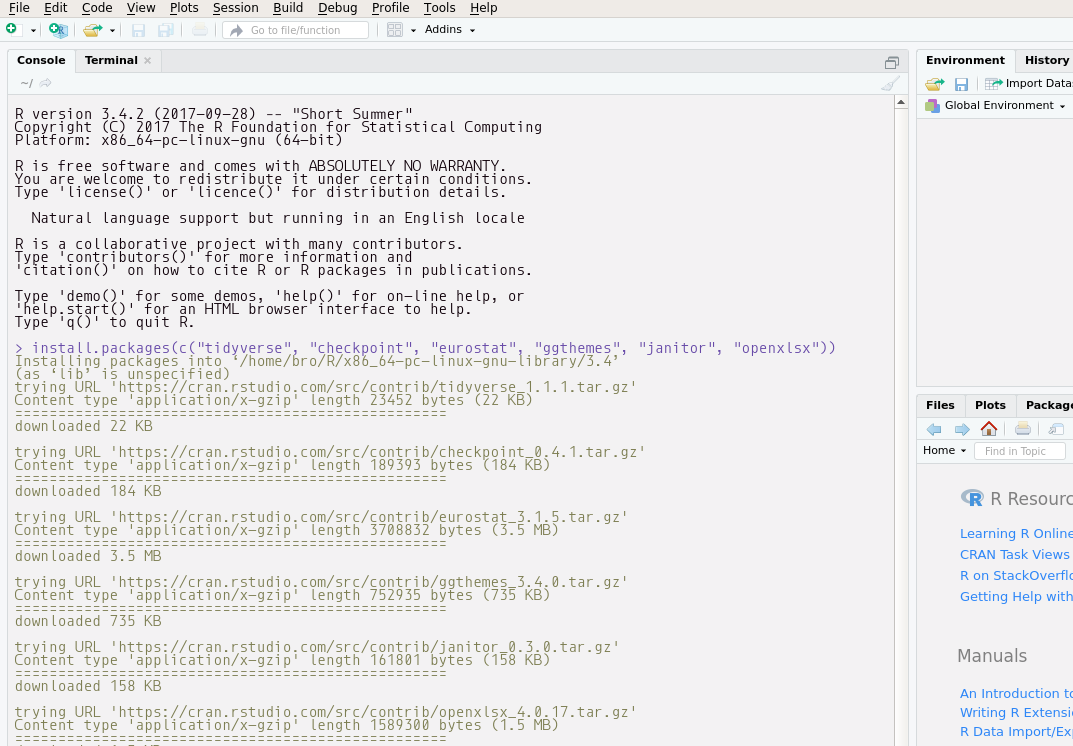
\includegraphics{pics/install_packages.png}

or go to the \textbf{Packages} pane and then click on \emph{Install}:

\includegraphics{pics/rstudio_install_packages.gif}

\hypertarget{the-author}{%
\subsection*{The author}\label{the-author}}
\addcontentsline{toc}{subsection}{The author}

My name is Bruno Rodrigues and I program almost exclusively in R and have been teaching some R
courses for a few years now. I first started teaching for students at the University of Strasbourg
while working on my PhD.
These notes are an update of those I used at the time, plus a lot of things I've learned about R
since then in my jobs.
In my free time I like cooking, working out and \href{https://www.brodrigues.co}{blogging}, while listening to
\href{http://www.fipradio.fr/player}{Fip} or \href{https://www.youtube.com/watch?v=u5qwtO_ABPM}{Vaporwave}.
I also like to get my butt handed to me by playing roguelikes
such as \href{http://nethack.wikia.com/wiki/NetHack}{NetHack}, for which I wrote a
\href{https://github.com/b-rodrigues/nethack}{package} that contains functions to analyze the data that
is saved on your computer after you win or lose (it will be lose 99\% of the time) the game.

You can follow me on \href{https://www.twitter.com/brodriguesco}{twitter}, I tweet mostly about R or
what's happening in Luxembourg.

\hypertarget{getting-to-know-rstudio}{%
\section{Getting to know RStudio}\label{getting-to-know-rstudio}}

Placeholder

\hypertarget{panes}{%
\subsection{Panes}\label{panes}}

\hypertarget{console}{%
\subsection{Console}\label{console}}

\hypertarget{scripts}{%
\subsection{Scripts}\label{scripts}}

\hypertarget{the-help-pane}{%
\subsubsection{The help pane}\label{the-help-pane}}

\hypertarget{the-environment-pane}{%
\subsubsection{The Environment pane}\label{the-environment-pane}}

\hypertarget{options}{%
\subsection{Options}\label{options}}

\hypertarget{keyboard-shortcuts}{%
\subsection{Keyboard shortcuts}\label{keyboard-shortcuts}}

\hypertarget{projects}{%
\subsection{Projects}\label{projects}}

\hypertarget{history}{%
\subsection{History}\label{history}}

\hypertarget{plots}{%
\subsection{Plots}\label{plots}}

\hypertarget{addins}{%
\subsection{Addins}\label{addins}}

\hypertarget{packages}{%
\subsection{Packages}\label{packages}}

\hypertarget{exercises}{%
\subsection{Exercises}\label{exercises}}

\hypertarget{exercise-1}{%
\subsubsection*{Exercise 1}\label{exercise-1}}
\addcontentsline{toc}{subsubsection}{Exercise 1}

\hypertarget{objects-types-and-useful-r-functions-to-get-started}{%
\section{Objects, types and useful R functions to get started}\label{objects-types-and-useful-r-functions-to-get-started}}

Placeholder

\hypertarget{the-numeric-class}{%
\subsection{\texorpdfstring{The \texttt{numeric} class}{The numeric class}}\label{the-numeric-class}}

\hypertarget{the-character-class}{%
\subsection{\texorpdfstring{The \texttt{character} class}{The character class}}\label{the-character-class}}

\hypertarget{the-factor-class}{%
\subsection{\texorpdfstring{The \texttt{factor} class}{The factor class}}\label{the-factor-class}}

\hypertarget{the-date-class}{%
\subsection{\texorpdfstring{The \texttt{Date} class}{The Date class}}\label{the-date-class}}

\hypertarget{the-logical-class}{%
\subsection{\texorpdfstring{The \texttt{logical} class}{The logical class}}\label{the-logical-class}}

\hypertarget{vectors-and-matrices}{%
\subsection{Vectors and matrices}\label{vectors-and-matrices}}

\hypertarget{the-c-function}{%
\subsubsection{\texorpdfstring{The \texttt{c()} function}{The c() function}}\label{the-c-function}}

\hypertarget{cbind-and-rbind}{%
\subsubsection{\texorpdfstring{\texttt{cbind()} and \texttt{rbind()}}{cbind() and rbind()}}\label{cbind-and-rbind}}

\hypertarget{the-matrix-class}{%
\subsubsection{\texorpdfstring{The \texttt{matrix} class}{The matrix class}}\label{the-matrix-class}}

\hypertarget{the-list-class}{%
\subsection{\texorpdfstring{The \texttt{list} class}{The list class}}\label{the-list-class}}

\hypertarget{the-data.frame-and-tibble-classes}{%
\subsection{\texorpdfstring{The \texttt{data.frame} and \texttt{tibble} classes}{The data.frame and tibble classes}}\label{the-data.frame-and-tibble-classes}}

\hypertarget{formulas}{%
\subsection{Formulas}\label{formulas}}

\hypertarget{models}{%
\subsection{Models}\label{models}}

\hypertarget{null-na-and-nan}{%
\subsection{NULL, NA and NaN}\label{null-na-and-nan}}

\hypertarget{useful-functions-to-get-you-started}{%
\subsection{Useful functions to get you started}\label{useful-functions-to-get-you-started}}

\hypertarget{sequences}{%
\subsubsection{Sequences}\label{sequences}}

\hypertarget{basic-string-manipulation}{%
\subsubsection{Basic string manipulation}\label{basic-string-manipulation}}

\hypertarget{exercises-1}{%
\subsection{Exercises}\label{exercises-1}}

\hypertarget{exercise-1-1}{%
\subsubsection*{Exercise 1}\label{exercise-1-1}}
\addcontentsline{toc}{subsubsection}{Exercise 1}

\hypertarget{exercise-2}{%
\subsubsection*{Exercise 2}\label{exercise-2}}
\addcontentsline{toc}{subsubsection}{Exercise 2}

\hypertarget{exercise-3}{%
\subsubsection*{Exercise 3}\label{exercise-3}}
\addcontentsline{toc}{subsubsection}{Exercise 3}

\hypertarget{exercise-4}{%
\subsubsection*{Exercise 4}\label{exercise-4}}
\addcontentsline{toc}{subsubsection}{Exercise 4}

\hypertarget{exercise-5}{%
\subsubsection*{Exercise 5}\label{exercise-5}}
\addcontentsline{toc}{subsubsection}{Exercise 5}

\hypertarget{exercise-6}{%
\subsubsection*{Exercise 6}\label{exercise-6}}
\addcontentsline{toc}{subsubsection}{Exercise 6}

\hypertarget{exercise-7}{%
\subsubsection*{Exercise 7}\label{exercise-7}}
\addcontentsline{toc}{subsubsection}{Exercise 7}

\hypertarget{exercise-8}{%
\subsubsection*{Exercise 8}\label{exercise-8}}
\addcontentsline{toc}{subsubsection}{Exercise 8}

\hypertarget{reading-and-writing-data}{%
\section{Reading and writing data}\label{reading-and-writing-data}}

Placeholder

\hypertarget{the-swiss-army-knife-of-data-import-and-export-rio}{%
\subsection{\texorpdfstring{The swiss army knife of data import and export: \texttt{\{rio\}}}{The swiss army knife of data import and export: \{rio\}}}\label{the-swiss-army-knife-of-data-import-and-export-rio}}

\hypertarget{writing-any-object-to-disk}{%
\subsection{Writing any object to disk}\label{writing-any-object-to-disk}}

\hypertarget{using-rstudio-projects-to-manage-paths}{%
\subsection{Using RStudio projects to manage paths}\label{using-rstudio-projects-to-manage-paths}}

\hypertarget{descriptive-statistics-and-data-manipulation}{%
\section{Descriptive statistics and data manipulation}\label{descriptive-statistics-and-data-manipulation}}

Placeholder

\hypertarget{a-data-exploration-exercice-using-base-r}{%
\subsection{\texorpdfstring{A data exploration exercice using \emph{base} R}{A data exploration exercice using base R}}\label{a-data-exploration-exercice-using-base-r}}

\hypertarget{smoking-is-bad-for-you-but-pipes-are-your-friend}{%
\subsection{Smoking is bad for you, but pipes are your friend}\label{smoking-is-bad-for-you-but-pipes-are-your-friend}}

\hypertarget{the-tidyverses-enfant-prodige-dplyr}{%
\subsection{\texorpdfstring{The \texttt{\{tidyverse\}}'s \emph{enfant prodige}: \texttt{\{dplyr\}}}{The \{tidyverse\}'s enfant prodige: \{dplyr\}}}\label{the-tidyverses-enfant-prodige-dplyr}}

\hypertarget{a-first-taste-of-data-manipulation-with-dplyr}{%
\subsubsection{\texorpdfstring{A first taste of data manipulation with \texttt{\{dplyr\}}}{A first taste of data manipulation with \{dplyr\}}}\label{a-first-taste-of-data-manipulation-with-dplyr}}

\hypertarget{filter-the-rows-of-a-dataset-with-filter}{%
\subsubsection{\texorpdfstring{Filter the rows of a dataset with \texttt{filter()}}{Filter the rows of a dataset with filter()}}\label{filter-the-rows-of-a-dataset-with-filter}}

\hypertarget{select-columns-with-select}{%
\subsubsection{\texorpdfstring{Select columns with \texttt{select()}}{Select columns with select()}}\label{select-columns-with-select}}

\hypertarget{group-the-observations-of-your-dataset-with-group_by}{%
\subsubsection{\texorpdfstring{Group the observations of your dataset with \texttt{group\_by()}}{Group the observations of your dataset with group\_by()}}\label{group-the-observations-of-your-dataset-with-group_by}}

\hypertarget{groups-country-18}{%
\subsection{\# Groups: country {[}18{]}}\label{groups-country-18}}

\hypertarget{get-summary-statistics-with-summarise}{%
\subsubsection{\texorpdfstring{Get summary statistics with \texttt{summarise()}}{Get summary statistics with summarise()}}\label{get-summary-statistics-with-summarise}}

\hypertarget{adding-columns-with-mutate-and-transmute}{%
\subsubsection{\texorpdfstring{Adding columns with \texttt{mutate()} and \texttt{transmute()}}{Adding columns with mutate() and transmute()}}\label{adding-columns-with-mutate-and-transmute}}

\hypertarget{joining-tibbles-with-full_join-left_join-right_join-and-all-the-others}{%
\subsubsection{\texorpdfstring{Joining \texttt{tibble}s with \texttt{full\_join()}, \texttt{left\_join()}, \texttt{right\_join()} and all the others}{Joining tibbles with full\_join(), left\_join(), right\_join() and all the others}}\label{joining-tibbles-with-full_join-left_join-right_join-and-all-the-others}}

\hypertarget{reshaping-data-with-tidyr}{%
\subsection{\texorpdfstring{Reshaping data with \texttt{tidyr}}{Reshaping data with tidyr}}\label{reshaping-data-with-tidyr}}

\hypertarget{pivot_wider-and-pivot_longer}{%
\subsubsection{\texorpdfstring{\texttt{pivot\_wider()} and \texttt{pivot\_longer()}}{pivot\_wider() and pivot\_longer()}}\label{pivot_wider-and-pivot_longer}}

\hypertarget{spread-and-gather}{%
\subsubsection{\texorpdfstring{\texttt{spread()} and \texttt{gather()}}{spread() and gather()}}\label{spread-and-gather}}

\hypertarget{fill-and-full_seq}{%
\subsubsection{\texorpdfstring{\texttt{fill()} and \texttt{full\_seq()}}{fill() and full\_seq()}}\label{fill-and-full_seq}}

\hypertarget{put-order-in-your-columns-with-separate-unite-and-in-your-rows-with-separate_rows}{%
\subsubsection{\texorpdfstring{Put order in your columns with \texttt{separate()}, \texttt{unite()}, and in your rows with \texttt{separate\_rows()}}{Put order in your columns with separate(), unite(), and in your rows with separate\_rows()}}\label{put-order-in-your-columns-with-separate-unite-and-in-your-rows-with-separate_rows}}

\hypertarget{a-sneak-peek-to-chapter-8-nest}{%
\subsubsection{\texorpdfstring{A sneak peek to Chapter 8; \texttt{nest()}}{A sneak peek to Chapter 8; nest()}}\label{a-sneak-peek-to-chapter-8-nest}}

\hypertarget{scoped-tidyverse-verbs}{%
\subsection{\texorpdfstring{Scoped \texttt{\{tidyverse\}} verbs}{Scoped \{tidyverse\} verbs}}\label{scoped-tidyverse-verbs}}

\hypertarget{filter_-select_-and-rename_-group_by_}{%
\subsubsection{\texorpdfstring{filter\_\emph{()
\#\#\# select\_*() and rename\_*()
\#\#\# group\_by\_}()}{filter\_() \#\#\# select\_*() and rename\_*() \#\#\# group\_by\_()}}\label{filter_-select_-and-rename_-group_by_}}

\hypertarget{summarise_}{%
\subsubsection{summarise\_()}\label{summarise_}}

\hypertarget{mutate_-other-useful-tidyverse-functions-if_else-case_when-and-recode-lead-and-lag-ntile-arrange-tally-and-count-special-packages-for-special-kinds-of-data-forcats-lubridate-and-stringr-get-your-dates-right-with-lubridate-defining-dates-the-tidy-way-data-manipulation-with-dates-arithmetic-with-dates-manipulate-strings-with-stringr-getting-text-data-into-rstudio-detecting-getting-the-position-and-locating-strings-splitting-strings-matching-strings-searching-and-replacing-strings-exctracting-or-removing-strings-tidy-data-frames-with-tibble-creating-tibbles-list-columns-going-beyond-descriptive-statistics-and-data-manipulation-exercises-exercise-1---exercise-2---exercise-3--}{%
\subsubsection{\texorpdfstring{mutate\_*()
\#\# Other useful \texttt{\{tidyverse\}} functions
\#\#\# \texttt{if\_else()}, \texttt{case\_when()} and \texttt{recode()}
\#\#\# \texttt{lead()} and \texttt{lag()}
\#\#\# \texttt{ntile()}
\#\#\# \texttt{arrange()}
\#\#\# \texttt{tally()} and \texttt{count()}
\#\# Special packages for special kinds of data: \texttt{\{forcats\}}, \texttt{\{lubridate\}}, and \texttt{\{stringr\}}
\#\#\# 🐈🐈🐈🐈
\#\#\# Get your dates right with \texttt{\{lubridate\}}
\#\#\#\# Defining dates, the tidy way
\#\#\#\# Data manipulation with dates
\#\#\#\# Arithmetic with dates
\#\#\# Manipulate strings with \texttt{\{stringr\}}
\#\#\#\# Getting text data into Rstudio
\#\#\#\# Detecting, getting the position and locating strings
\#\#\#\# Splitting strings
\#\#\#\# Matching strings
\#\#\#\# Searching and replacing strings
\#\#\#\# Exctracting or removing strings
\#\#\# Tidy data frames with \texttt{\{tibble\}}
\#\#\#\# Creating tibbles
\#\# List-columns
\#\# Going beyond descriptive statistics and data manipulation
\#\# Exercises
\#\#\# Exercise 1 \{-\}
\#\#\# Exercise 2 \{-\}
\#\#\# Exercise 3 \{-\}}{mutate\_*() \#\# Other useful \{tidyverse\} functions \#\#\# if\_else(), case\_when() and recode() \#\#\# lead() and lag() \#\#\# ntile() \#\#\# arrange() \#\#\# tally() and count() \#\# Special packages for special kinds of data: \{forcats\}, \{lubridate\}, and \{stringr\} \#\#\# 🐈🐈🐈🐈 \#\#\# Get your dates right with \{lubridate\} \#\#\#\# Defining dates, the tidy way \#\#\#\# Data manipulation with dates \#\#\#\# Arithmetic with dates \#\#\# Manipulate strings with \{stringr\} \#\#\#\# Getting text data into Rstudio \#\#\#\# Detecting, getting the position and locating strings \#\#\#\# Splitting strings \#\#\#\# Matching strings \#\#\#\# Searching and replacing strings \#\#\#\# Exctracting or removing strings \#\#\# Tidy data frames with \{tibble\} \#\#\#\# Creating tibbles \#\# List-columns \#\# Going beyond descriptive statistics and data manipulation \#\# Exercises \#\#\# Exercise 1 \{-\} \#\#\# Exercise 2 \{-\} \#\#\# Exercise 3 \{-\}}}\label{mutate_-other-useful-tidyverse-functions-if_else-case_when-and-recode-lead-and-lag-ntile-arrange-tally-and-count-special-packages-for-special-kinds-of-data-forcats-lubridate-and-stringr-get-your-dates-right-with-lubridate-defining-dates-the-tidy-way-data-manipulation-with-dates-arithmetic-with-dates-manipulate-strings-with-stringr-getting-text-data-into-rstudio-detecting-getting-the-position-and-locating-strings-splitting-strings-matching-strings-searching-and-replacing-strings-exctracting-or-removing-strings-tidy-data-frames-with-tibble-creating-tibbles-list-columns-going-beyond-descriptive-statistics-and-data-manipulation-exercises-exercise-1---exercise-2---exercise-3--}}

\hypertarget{graphs}{%
\section{Graphs}\label{graphs}}

Placeholder

\hypertarget{resources}{%
\subsection{Resources}\label{resources}}

\hypertarget{examples}{%
\subsection{Examples}\label{examples}}

\hypertarget{barplots}{%
\subsubsection{Barplots}\label{barplots}}

\hypertarget{scatter-plots}{%
\subsubsection{Scatter plots}\label{scatter-plots}}

\hypertarget{density}{%
\subsubsection{Density}\label{density}}

\hypertarget{line-plots}{%
\subsubsection{Line plots}\label{line-plots}}

\hypertarget{facets}{%
\subsubsection{Facets}\label{facets}}

\hypertarget{pie-charts}{%
\subsubsection{Pie Charts}\label{pie-charts}}

\hypertarget{adding-text-to-plots}{%
\subsubsection{Adding text to plots}\label{adding-text-to-plots}}

\hypertarget{customization}{%
\subsection{Customization}\label{customization}}

\hypertarget{changing-titles-axes-labels-options-mixing-geoms-and-changing-themes}{%
\subsubsection{Changing titles, axes labels, options, mixing geoms and changing themes}\label{changing-titles-axes-labels-options-mixing-geoms-and-changing-themes}}

\hypertarget{colour-schemes}{%
\subsubsection{Colour schemes}\label{colour-schemes}}

\hypertarget{saving-plots-to-disk}{%
\subsection{Saving plots to disk}\label{saving-plots-to-disk}}

\hypertarget{exercises-2}{%
\subsection{Exercises}\label{exercises-2}}

\hypertarget{exercise-1-2}{%
\subsubsection*{Exercise 1}\label{exercise-1-2}}
\addcontentsline{toc}{subsubsection}{Exercise 1}

\hypertarget{statistical-models}{%
\section{Statistical models}\label{statistical-models}}

Placeholder

\hypertarget{terminology}{%
\subsection{Terminology}\label{terminology}}

\hypertarget{fitting-a-model-to-data}{%
\subsection{Fitting a model to data}\label{fitting-a-model-to-data}}

\hypertarget{diagnostics}{%
\subsection{Diagnostics}\label{diagnostics}}

\hypertarget{interpreting-models}{%
\subsection{Interpreting models}\label{interpreting-models}}

\hypertarget{comparing-models}{%
\subsection{Comparing models}\label{comparing-models}}

\hypertarget{using-a-model-for-prediction}{%
\subsection{Using a model for prediction}\label{using-a-model-for-prediction}}

\hypertarget{beyond-linear-regression}{%
\subsection{Beyond linear regression}\label{beyond-linear-regression}}

\hypertarget{hyper-parameters}{%
\subsection{Hyper-parameters}\label{hyper-parameters}}

\hypertarget{ridge-regression}{%
\subsubsection{Ridge regression}\label{ridge-regression}}

\hypertarget{training-validating-and-testing-models}{%
\subsection{Training, validating, and testing models}\label{training-validating-and-testing-models}}

\hypertarget{set-up}{%
\subsubsection{Set up}\label{set-up}}

\hypertarget{bayesian-hyperparameter-optimization}{%
\subsubsection{Bayesian hyperparameter optimization}\label{bayesian-hyperparameter-optimization}}

\hypertarget{defining-your-own-functions}{%
\section{Defining your own functions}\label{defining-your-own-functions}}

Placeholder

\hypertarget{control-flow}{%
\subsection{Control flow}\label{control-flow}}

\hypertarget{if-else}{%
\subsubsection{If-else}\label{if-else}}

\hypertarget{for-loops}{%
\subsubsection{For loops}\label{for-loops}}

\hypertarget{while-loops}{%
\subsubsection{While loops}\label{while-loops}}

\hypertarget{writing-your-own-functions}{%
\subsection{Writing your own functions}\label{writing-your-own-functions}}

\hypertarget{declaring-functions-in-r}{%
\subsubsection{Declaring functions in R}\label{declaring-functions-in-r}}

\hypertarget{fibonacci-numbers}{%
\subsubsection{Fibonacci numbers}\label{fibonacci-numbers}}

\hypertarget{exercises-3}{%
\subsection{Exercises}\label{exercises-3}}

\hypertarget{exercise-1-3}{%
\subsubsection*{Exercise 1}\label{exercise-1-3}}
\addcontentsline{toc}{subsubsection}{Exercise 1}

\hypertarget{exercise-2-1}{%
\subsubsection*{Exercise 2}\label{exercise-2-1}}
\addcontentsline{toc}{subsubsection}{Exercise 2}

\hypertarget{exercise-3-1}{%
\subsubsection*{Exercise 3}\label{exercise-3-1}}
\addcontentsline{toc}{subsubsection}{Exercise 3}

\hypertarget{functions-that-take-functions-as-arguments-writing-your-own-higher-order-functions}{%
\subsection{Functions that take functions as arguments: writing your own higher-order functions}\label{functions-that-take-functions-as-arguments-writing-your-own-higher-order-functions}}

\hypertarget{functions-that-take-columns-of-data-as-arguments}{%
\subsection{Functions that take columns of data as arguments}\label{functions-that-take-columns-of-data-as-arguments}}

\hypertarget{the-enquo---approach}{%
\subsubsection{\texorpdfstring{The \texttt{enquo()\ -\ !!()} approach}{The enquo() - !!() approach}}\label{the-enquo---approach}}

\hypertarget{curly-curly-a-simplified-approach-to-the-enquo-and-framework}{%
\subsubsection{\texorpdfstring{Curly Curly, a simplified approach to the \texttt{enquo()} and \texttt{!!()} framework}{Curly Curly, a simplified approach to the enquo() and !!() framework}}\label{curly-curly-a-simplified-approach-to-the-enquo-and-framework}}

\hypertarget{functions-that-use-loops}{%
\subsection{Functions that use loops}\label{functions-that-use-loops}}

\hypertarget{anonymous-functions}{%
\subsection{Anonymous functions}\label{anonymous-functions}}

\hypertarget{exercises-4}{%
\subsection{Exercises}\label{exercises-4}}

\hypertarget{exercise-1-4}{%
\subsubsection*{Exercise 1}\label{exercise-1-4}}
\addcontentsline{toc}{subsubsection}{Exercise 1}

\hypertarget{exercise-2-2}{%
\subsubsection*{Exercise 2}\label{exercise-2-2}}
\addcontentsline{toc}{subsubsection}{Exercise 2}

\hypertarget{exercise-3-2}{%
\subsubsection*{Exercise 3}\label{exercise-3-2}}
\addcontentsline{toc}{subsubsection}{Exercise 3}

\hypertarget{exercise-4-1}{%
\subsubsection*{Exercise 4}\label{exercise-4-1}}
\addcontentsline{toc}{subsubsection}{Exercise 4}

\hypertarget{functional-programming}{%
\section{Functional programming}\label{functional-programming}}

Placeholder

\hypertarget{function-definitions}{%
\subsection{Function definitions}\label{function-definitions}}

\hypertarget{properties-of-functions}{%
\subsection{Properties of functions}\label{properties-of-functions}}

\hypertarget{functional-programming-with-purrr}{%
\subsection{\texorpdfstring{Functional programming with \texttt{\{purrr\}}}{Functional programming with \{purrr\}}}\label{functional-programming-with-purrr}}

\hypertarget{doing-away-with-loops-the-map-family-of-functions}{%
\subsubsection{\texorpdfstring{Doing away with loops: the \texttt{map*()} family of functions}{Doing away with loops: the map*() family of functions}}\label{doing-away-with-loops-the-map-family-of-functions}}

\hypertarget{reducing-with-purrr}{%
\subsubsection{\texorpdfstring{Reducing with \texttt{purrr}}{Reducing with purrr}}\label{reducing-with-purrr}}

\hypertarget{error-handling-with-safely-and-possibly}{%
\subsubsection{\texorpdfstring{Error handling with \texttt{safely()} and \texttt{possibly()}}{Error handling with safely() and possibly()}}\label{error-handling-with-safely-and-possibly}}

\hypertarget{partial-applications-with-partial}{%
\subsubsection{\texorpdfstring{Partial applications with \texttt{partial()}}{Partial applications with partial()}}\label{partial-applications-with-partial}}

\hypertarget{function-composition-using-compose}{%
\subsubsection{\texorpdfstring{Function composition using \texttt{compose}}{Function composition using compose}}\label{function-composition-using-compose}}

\hypertarget{type-safety-with-checkmate}{%
\subsubsection{\texorpdfstring{Type safety with \texttt{\{checkmate\}}}{Type safety with \{checkmate\}}}\label{type-safety-with-checkmate}}

\hypertarget{is_-as_}{%
\subsubsection{\texorpdfstring{\texttt{is\_*()} \texttt{as\_*()}}{is\_*() as\_*()}}\label{is_-as_}}

\hypertarget{transposing-lists}{%
\subsubsection{«Transposing lists»}\label{transposing-lists}}

\hypertarget{list-based-workflows-for-efficiency}{%
\subsection{List-based workflows for efficiency}\label{list-based-workflows-for-efficiency}}

\hypertarget{functional-programming-and-plotting}{%
\subsubsection{Functional programming and plotting}\label{functional-programming-and-plotting}}

\hypertarget{modeling-with-functional-programming}{%
\subsubsection{Modeling with functional programming}\label{modeling-with-functional-programming}}

\hypertarget{exercises-5}{%
\subsection{Exercises}\label{exercises-5}}

\hypertarget{exercise-1-5}{%
\subsubsection*{Exercise 1}\label{exercise-1-5}}
\addcontentsline{toc}{subsubsection}{Exercise 1}

\hypertarget{exercise-2-3}{%
\subsubsection*{Exercise 2}\label{exercise-2-3}}
\addcontentsline{toc}{subsubsection}{Exercise 2}

\hypertarget{package-development}{%
\section{Package development}\label{package-development}}

\hypertarget{why-you-need-to-write-your-own-package}{%
\subsection{Why you need to write your own package}\label{why-you-need-to-write-your-own-package}}

\hypertarget{unit-testing-your-package}{%
\subsection{Unit testing your package}\label{unit-testing-your-package}}

\hypertarget{further-topics}{%
\section{Further topics}\label{further-topics}}

\hypertarget{using-python-from-r-with-reticulate}{%
\subsection{\texorpdfstring{Using Python from R with \texttt{\{reticulate\}}}{Using Python from R with \{reticulate\}}}\label{using-python-from-r-with-reticulate}}

\hypertarget{generating-pdf-or-word-reports-with-r}{%
\subsection{Generating Pdf or Word reports with R}\label{generating-pdf-or-word-reports-with-r}}

\hypertarget{scraping-the-internet}{%
\subsection{Scraping the internet}\label{scraping-the-internet}}

\hypertarget{regular-expressions}{%
\subsection{Regular expressions}\label{regular-expressions}}

\hypertarget{setting-up-a-blog-with-blogdown}{%
\subsection{\texorpdfstring{Setting up a blog with \texttt{\{blogdown\}}}{Setting up a blog with \{blogdown\}}}\label{setting-up-a-blog-with-blogdown}}

\bibliography{book.bib,packages.bib}


\end{document}
